% begin module concavity-def
\begin{frame}
\frametitle{What Does $f''$ Say About $f$?}
$f$ and $g$ are both increasing functions on $(a,b)$, but they look different because they bend in different directions.
\begin{columns}[c]
\column{.5\textwidth}
\psset{xunit=0.6cm, yunit=0.6cm}
\begin{pspicture}(-5, -5)(5,5) 
\psframe*[linecolor=white](-5,-5)(5,5) 
\psaxes[ticks=none, labels=none]{<->}(0,0)(-0.5,-0.6)(4,3.8)
%Function formula: 1/2+1/4 ((-1+x)^{2})+1/4 (x) 
\psplot[linecolor=red, plotpoints=1000]{-0.5}{4}{x 0.25 mul x -1 add 2 exp 0.25 mul add 0.5 add }
\tiny
\rput(1, 2){$y=f(x)$}
\uncover<3>{
%Function formula: -1/10 (x)+291/400 
\psplot[linecolor=blue, plotpoints=1000]{-0.5}{4}{0.7275 x -0.1 mul add }
}
\uncover<4->{
%Function formula: -1/10 (x)+291/400 
\psplot[linecolor=blue, plotpoints=1000]{0}{0.6}{0.7275 x -0.1 mul add } 
}
\uncover<3->{
\psFullDot{0.3}{0.6975}
}

\uncover<4>{
%Function formula: 2/5 (x)+131/400 
\psplot[linecolor=blue, plotpoints=1000]{-0.5}{4}{0.3275 x 0.4 mul add } 
}
\uncover<5->{
%Function formula: 2/5 (x)+131/400 
\psplot[linecolor=blue, plotpoints=1000]{1}{1.6}{0.3275 x 0.4 mul add } 
}
\uncover<4->{
\psFullDot{1.3}{0.8475}
}

\uncover<5>{
%Function formula: 9/10 (x)-229/400 
\psplot[linecolor=blue, plotpoints=1000]{0.080555556}{4}{-0.5725 x 0.9 mul add } 
}
\uncover<6->{
%Function formula: 9/10 (x)-229/400 
\psplot[linecolor=blue, plotpoints=1000]{2}{2.6}{-0.5725 x 0.9 mul add } 
}
\uncover<5->{
\psFullDot{2.3}{1.4975}
}

\uncover<6>{
%Function formula: 7/5 (x)-789/400 
\psplot[linecolor=blue, plotpoints=1000]{1.051785714}{4}{-1.9725 x 1.4 mul add } 
}
\uncover<7->{
%Function formula: 7/5 (x)-789/400 
\psplot[linecolor=blue, plotpoints=1000]{3}{3.6}{-1.9725 x 1.4 mul add } 
}
\uncover<6->{
\psFullDot{3.3}{2.6475}
}
\end{pspicture} 
%\ \only<handout:0| -2>{%
%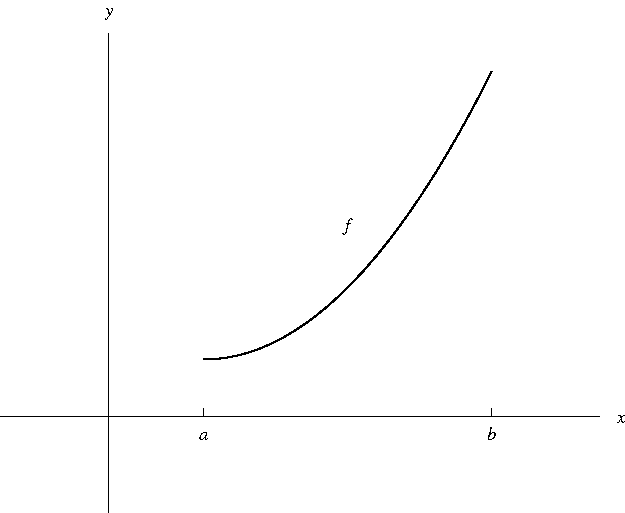
\includegraphics[height=3.5cm]{curve-sketching/pictures/04-03-concaveupa.pdf}%
%}%
%\only<handout:0| 3>{%
%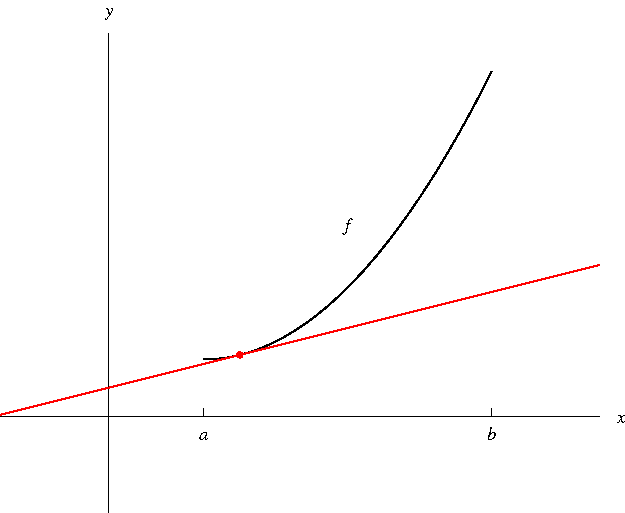
\includegraphics[height=3.5cm]{curve-sketching/pictures/04-03-concaveupb.pdf}%
%}%
%\only<handout:0| 4>{%
%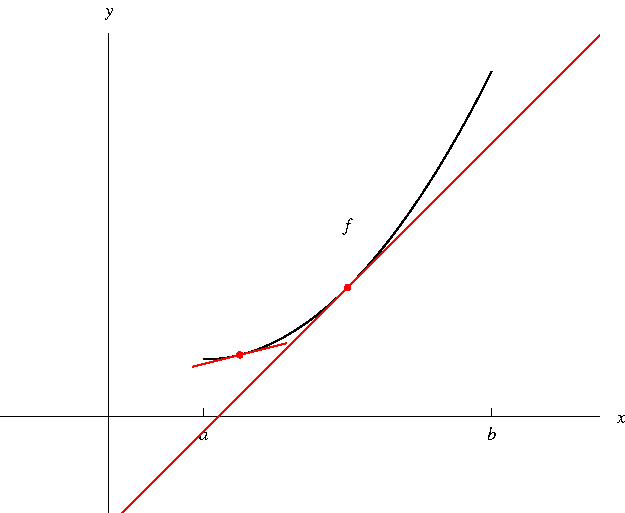
\includegraphics[height=3.5cm]{curve-sketching/pictures/04-03-concaveupc.pdf}%
%}%
%\only<handout:0| 5>{%
%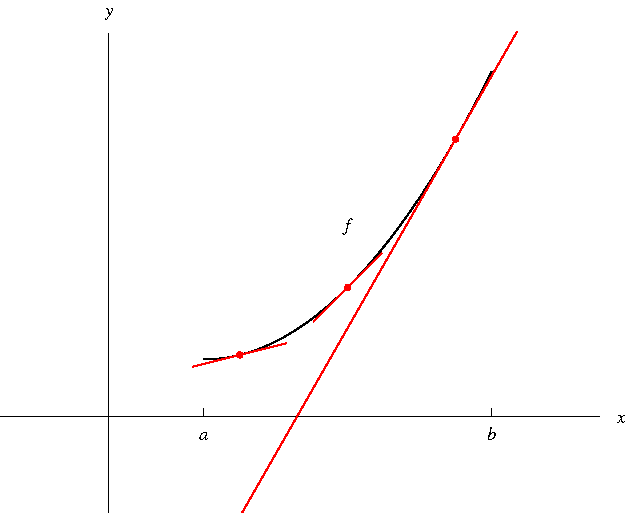
\includegraphics[height=3.5cm]{curve-sketching/pictures/04-03-concaveupd.pdf}%
%}%
%\only<6->{%
%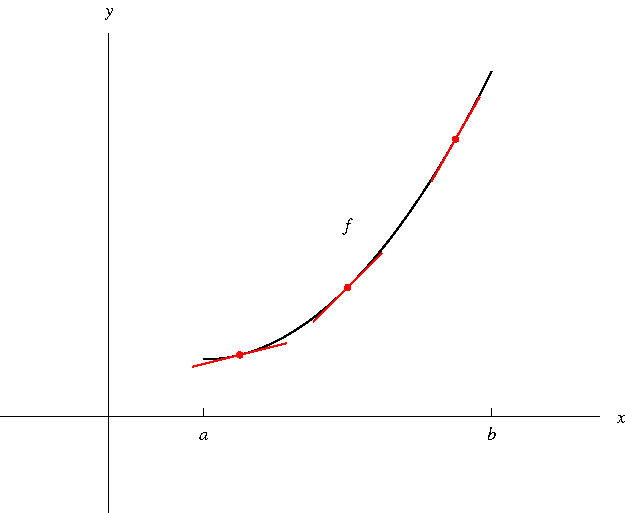
\includegraphics[height=3.5cm]{curve-sketching/pictures/04-03-concaveupe.pdf}%
%}%


%\begin{center}
\ \ \ \ \ \ \ \ \ \uncover<6->{Concave up}
%\end{center}
\column{.5\textwidth}
\psset{xunit=0.6cm, yunit=0.6cm}
\begin{pspicture}(-5, -5)(5,5) 
\psframe*[linecolor=white](-5,-5)(5,5) 
\psaxes[ticks=none, labels=none]{<->}(0,0)(-0.5,-0.6)(4,3.8)
\tiny
\rput(2, 1){$y=g(x)$}
%Function formula: 11/4-1/4 ((-3+x)^{2})-1/4 (x) 
\psplot[linecolor=red, plotpoints=1000]{-0.5}{4}{x -0.25 mul x -3 add 2 exp -0.25 mul add 2.75 add }

\uncover<3>{
%Function formula: 11/10 (x)+209/400 
\psplot[linecolor=blue, plotpoints=1000]{-0.5}{2.979}{0.5225 x 1.1 mul add }
}
\uncover<4->{ 
%Function formula: 11/10 (x)+209/400 
\psplot[linecolor=blue, plotpoints=1000]{0}{0.6}{0.5225 x 1.1 mul add } 
}
\uncover<3->{
\psFullDot{0.3}{0.8525}
}
\uncover<4>{
%Function formula: 3/5 (x)+369/400 
\psplot[linecolor=blue, plotpoints=1000]{-0.5}{4}{0.9225 x 0.6 mul add } 
}
\uncover<5->{
%Function formula: 3/5 (x)+369/400 
\psplot[linecolor=blue, plotpoints=1000]{1}{1.6}{0.9225 x 0.6 mul add } 
}
\uncover<4->{
\psFullDot{1.3}{1.7025}
}

\uncover<5>{
%Function formula: 1/10 (x)+729/400 
\psplot[linecolor=blue, plotpoints=1000]{-0.5}{4}{1.8225 x 0.1 mul add } 
}
\uncover<6->{
%Function formula: 1/10 (x)+729/400 
\psplot[linecolor=blue, plotpoints=1000]{2}{2.6}{1.8225 x 0.1 mul add } 
}
\uncover<5->{
\psFullDot{2.3}{2.0525}
}
\uncover<6>{
%Function formula: -2/5 (x)+1289/400 
\psplot[linecolor=blue, plotpoints=1000]{-0.5}{4}{3.2225 x -0.4 mul add } 
}
\uncover<7->{
%Function formula: -2/5 (x)+1289/400 
\psplot[linecolor=blue, plotpoints=1000]{3}{3.6}{3.2225 x -0.4 mul add } 
}
\uncover<6->{
\psFullDot{3.3}{1.9025}
}
\end{pspicture} 
%\ \only<handout:0| -2>{%
%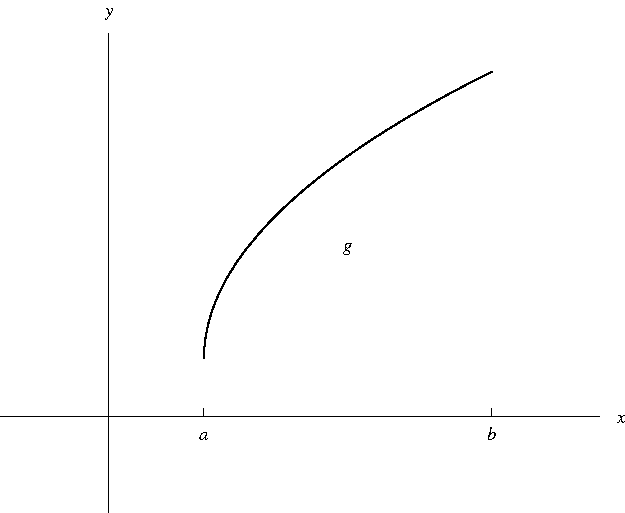
\includegraphics[height=3.5cm]{curve-sketching/pictures/04-03-concavedowna.pdf}%
%}%
%\only<handout:0| 3>{%
%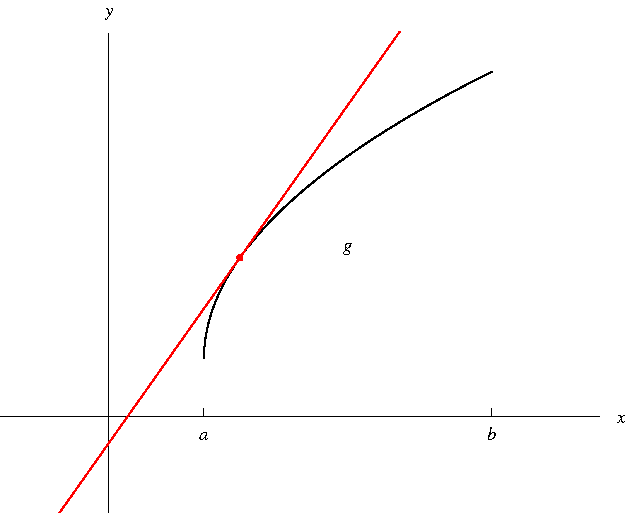
\includegraphics[height=3.5cm]{curve-sketching/pictures/04-03-concavedownb.pdf}%
%}%
%\only<handout:0| 4>{%
%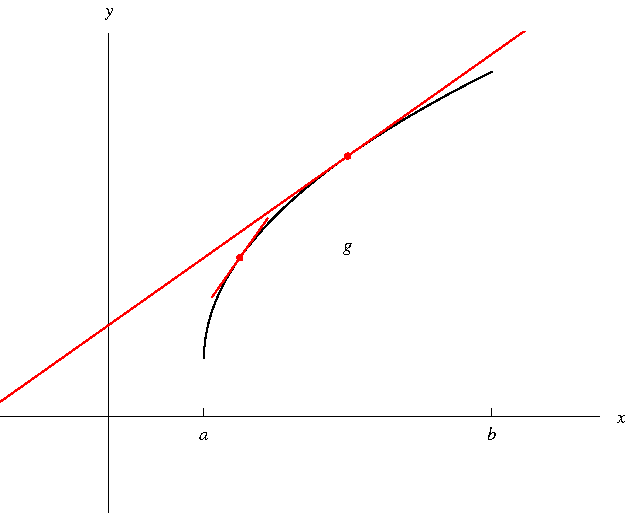
\includegraphics[height=3.5cm]{curve-sketching/pictures/04-03-concavedownc.pdf}%
%}%
%\only<handout:0| 5>{%
%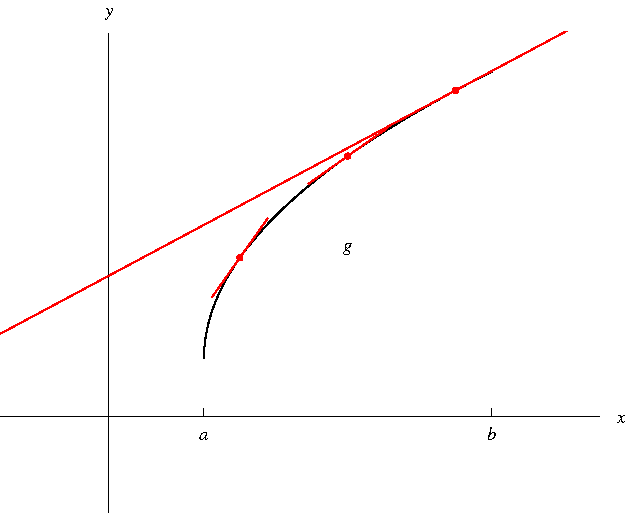
\includegraphics[height=3.5cm]{curve-sketching/pictures/04-03-concavedownd.pdf}%
%}%
%\only<6->{%
%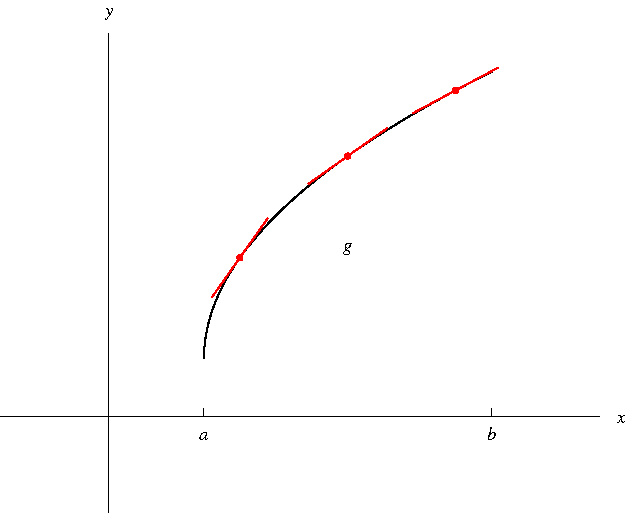
\includegraphics[height=3.5cm]{curve-sketching/pictures/04-03-concavedowne.pdf}%
%}%


%\begin{center}
\ \ \ \ \ \ \ \ \ \uncover<6->{Concave down}
%\end{center}
\end{columns}
\uncover<2-7>{%
\begin{definition}[Concave Up/Concave Down]
\color{gray} A function is called concave up/down if the line segment between any two points lies above/below its graph. \color{black}
Suppose $f$ is a differentiable function. If $f$ lies above all of its tangents on an interval $I$, then  we call it concave up on $I$.  If $f$ lies below all of its tangents on $I$, it we call it concave down on $I$.
\end{definition}
}%
\end{frame}
% end module concavity-def
